%%% LaTeX-Vorlage Version 2.0 %%%

% TODO: individuelle Einstellungen (Name, Titel etc.)
% -> bitte in Konfigurationsdatei anpassen
%%%%
%
% Zentrale Konfigurationsdatei
%
% In dieser Datei sind eine Reihe verpflichtender Einstellungen 
% (Nr. 1 bis 6) vorzunehmen.
%
% Die Einstellungen unter Nr. 7 bis 11 können im Regelfall unverändert
% belassen werden. Ausnahmen sind:
%  - Ihre Arbeit ist in englischer Sprache verfasst (Nr. 7)
%  - der Titel Ihrer Arbeit ist sehr lang, so dass er nicht auf das
%    Deckblatt passt oder anders umgebrochen werden soll (Nr. 8 und 9)
%  - es soll ein besonderes Abgabedatum angegeben werden (Nr. 10)
%  - Sie benötigen einen Vertraulichkeitsvermerk (Nr. 11)
%
%%%%


% TODO 1. Typ der Arbeit (für Titelseite und Metadaten)
% Zutreffendes auswählen:

%\newcommand{\typMeinerArbeit}{PA1} 
%\newcommand{\typMeinerArbeit}{PA2} 
\newcommand{\typMeinerArbeit}{Seminararbeit} 
%\newcommand{\typMeinerArbeit}{BA} 

% TODO 2. Vorname, Name der Autorin/des Autors (für Deckblatt und Metadaten)
\newcommand{\meinName}{Leonard Eckert, David Kreismann, Tobias Schnarr und Nico Wagner}

% TODO 3. Kurs eintragen
\newcommand{\meinKurs}{WWI2022F}

% TODO 4. Titel der Arbeit (für Deckblatt, ehrenwörtliche Erklärung und Metadaten, ohne Umbrüche angeben)
\newcommand{\themaMeinerArbeit}{Entwicklung einer Webanwendung zur automatisierten Veröffentlichung von Instagram-Beiträgen}



% OPTIONALE Einstellungen

% 7. Arbeit in Englisch
% (nur ändern, falls Ihre Arbeit in englischer Sprache geschrieben ist)
\newcommand{\meineSprache}{DE}	% Standard-Einstellung
% \newcommand{\meineSprache}{EN}	% für Arbeiten in englischer Sprache

% 8. Schriftgröße des Titels auf Deckblatt
% (nur ändern, falls Sie einen sehr langen Titel haben)
% Zutreffendes auswählen:
\newcommand{\schriftgroesseTitel}{\LARGE}   % Standard-Einstellung
%\newcommand{\schriftgroesseTitel}{\Large}  % bei sehr langen Titeln

% 9. Titel mit Umbrüchen für Deckblatt
% (nur ändern, falls Sie den Zeilenumbruch selbst beeinflussen möchten)
\newcommand{\titelAufDeckblatt}{\themaMeinerArbeit}		% Standard-Einstellung
%\newcommand{\titelAufDeckblatt}{Herausforderungen der Digitalisierung im globalen Wettbewerb von Industrieunternehmen \\ -- eine vergleichende Untersuchung unter Berücksichtigung aktueller und weniger aktueller Forschungsmethoden \\ am Beispiel der Firma Melanie Müller und Söhne AG} % explizite Angabe

% 10. Abgabedatum anpassen
% Zutreffendes auswählen:
\newcommand{\abgabeDatum}{\today}  		% Standard-Einstellung
%\newcommand{\abgabeDatum}{18.11.2024}  % falls nicht aktuelles Datum

% 11. Vertraulichkeitsvermerk
% (nur ändern, falls Ihre Arbeit einen Vertraulichkeitsvermerk tragen soll)
\newcommand{\hatVermerk}{nein}  	% Standard-Einstellung
%\newcommand{\hatVermerk}{ja}  	% falls Vertraulichkeitsvermerk


% Grundlegende Dokumenteneigenschaften gemäß DHBW-Vorgaben
\documentclass[a4paper,fontsize=11pt,oneside,parskip=half,headings=normal,listof=no chaptergap]{scrreprt} 
% \usepackage{showframe} % nur für Kontrolle der Ränder 

%%% Präambel einbinden (mit Festlegungen gemäß DHBW-Vorgaben) %%%
%%% Präambel %%%
% hier sollten keine Änderungen erforderlich sein
%
\usepackage{ifthen}           % für Umschaltung DE/EN
\newcommand{\DEoEN}[2]{\ifthenelse{\equal{\meineSprache}{DE}}{#1}{#2}}

\usepackage[utf8]{inputenc}   % Zeichencodierung UTF-8 für Eingabe-Dateien
\usepackage[T1]{fontenc}      % Darstellung von Umlauten im PDF
\usepackage{amsmath} % for math
\usepackage{multicol} % for multiple columns
\usepackage{booktabs} % for table formation
\usepackage{caption} % for captions in the appendix
\renewcommand{\theequation}{\arabic{equation}} % disable chapter-based numbering
\usepackage{float} % for figures
\usepackage{array} % for tables

\usepackage{listings}         % für Einbindung von Code-Listings
\lstset{numbers=left,numberstyle=\tiny,numbersep=5pt,texcl=true}
\lstset{literate=             % erlaubt Sonderzeichen in Code-Listings 
{Ö}{{\"O}}1
{Ä}{{\"A}}1
{Ü}{{\"U}}1
{ß}{{\ss}}2
{ü}{{\"u}}1
{ä}{{\"a}}1
{ö}{{\"o}}1
{€}{{\euro}}1
}

\usepackage[
  inner=35mm,outer=15mm,top=25mm,
  bottom=20mm,foot=12mm,includefoot
]{geometry}                 % Einstellungen für Ränder

\DEoEN{
  \usepackage[ngerman]{babel} % Spracheinstellungen Deutsch
  \usepackage[babel,german=quotes]{csquotes} % deutsche Anf.zeichen
}{
 \usepackage[english]{babel} % Spracheinstellungen Englisch
 \usepackage[babel,english=british]{csquotes} % englische Anf.zeichen
}

\usepackage{enumerate}      % anpassbare Nummerier./Aufz.
\usepackage{graphicx}       % Einbinden von Grafiken
\usepackage[onehalfspacing]{setspace} % anderthalbzeilig

\usepackage{blindtext}      % Textgenerierung für Testzwecke
\usepackage{color}          % Verwendung von Farbe 

\usepackage{acronym}        % für ein Abkürzungsverzeichnis

\usepackage[                % Biblatex
  backend=biber,
  bibstyle=_dhbw_authoryear,maxbibnames=99,
  citestyle=authoryear,     
  uniquename=true, useprefix=true,
  bibencoding=utf8]{biblatex}
%kein Punkt am Ende bei \footcite
%http://www.golatex.de/footcite-ohne-punkt-am-schluss-t4865.html
\renewcommand{\bibfootnotewrapper}[1]{\bibsentence#1}


%Reihenfolge der Autorennamen
%   
% http://golatex.de/viewtopic,p,80448.html#80448
% Argumente: siehe http://texwelt.de/blog/modifizieren-eines-biblatex-stils/
\DeclareNameFormat{sortname}{% Bibliographie
  \ifnum\value{uniquename}=0 % Normalfall
    \ifuseprefix%
      {%
         \usebibmacro{name:family-given}
           {\namepartfamily}
           {\namepartgiveni}
           {\namepartprefix}
           {\namepartsuffixi}%
       }
      {%
         \usebibmacro{name:family-given}
           {\namepartfamily}
           {\namepartgiveni}
           {\namepartprefixi}
           {\namepartsuffixi}%
       }%
  \fi
  \ifnum\value{uniquename}=1% falls nicht eindeutig, abgek. Vorname 
      {%
         \usebibmacro{name:family-given}
           {\namepartfamily}
           {\namepartgiveni}
           {\namepartprefix}
           {\namepartsuffix}%
       }%
  \fi
  \ifnum\value{uniquename}=2% falls nicht eindeutig, ganzer Vorname 
      {%
         \usebibmacro{name:family-given}
           {\namepartfamily}
           {\namepartgiven}
           {\namepartprefix}
           {\namepartsuffix}%
       }%
  \fi   
  \usebibmacro{name:andothers}}

\DeclareNameFormat{labelname}{% für Zitate
  \ifnum\value{uniquename}=0 % Normalfall
    \ifuseprefix%
      {%
         \usebibmacro{name:family-given}
           {\namepartfamily}
           {\empty}
           {\namepartprefix}
           {\namepartsuffixi}%
       }
      {%
         \usebibmacro{name:family-given}
           {\namepartfamily}
           {\empty}
           {\namepartprefixi}
           {\namepartsuffixi}%
       }%
  \fi
  \ifnum\value{uniquename}=1% falls nicht eindeutig, abgek. Vorname 
      {%
         \usebibmacro{name:family-given}
           {\namepartfamily}
           {\namepartgiveni}
           {\namepartprefix}
           {\namepartsuffix}%
       }%
  \fi
  \ifnum\value{uniquename}=2% falls nicht eindeutig, ganzer Vorname 
      {%
         \usebibmacro{name:family-given}
           {\namepartfamily}
           {\namepartgiven}
           {\namepartprefix}
           {\namepartsuffix}%
       }%
  \fi   
  \usebibmacro{name:andothers}}
      
  
\DeclareFieldFormat{extrayear}{% = the 'a' in 'Jones 1995a'
  \iffieldnums{labelyear}
    {\mknumalph{#1}}
    {\mknumalph{#1}}}        

\renewcommand*{\multinamedelim}{\addslash}
\renewcommand*{\finalnamedelim}{\addslash}
\renewcommand*{\multilistdelim}{\addslash}
\renewcommand*{\finallistdelim}{\addslash}

\renewcommand{\nameyeardelim}{~}

% Literaturverzeichnis: Doppelpunkt zwischen Name (Jahr): Rest 
% http://de.comp.text.tex.narkive.com/Tn1HUIXB/biblatex-authoryear-und-doppelpunkt
\renewcommand{\labelnamepunct}{\addcolon\addspace}

% damit die Darstellung für Vollzitate von Primärquellen in 
% Fußnoten später auf "nicht fett" geändert werden kann 
% (nur für Zitate von Sekundärliteratur relevant)
\newcommand{\textfett}[1]{\textbf{#1}}

% für Zitate von Sekundärliteratur:
\newcommand{\footcitePrimaerSekundaer}[4]{%
  \renewcommand{\textfett}[1]{##1}%
  \footnote{\fullcite[#2]{#1}, \DEoEN{zitiert nach}{as cited in} \cite[#4]{#3}}%  
  \renewcommand{\textfett}[1]{\textbf{##1}}%
}

% Im Literaturverzeichnis: Autor (Jahr) fett
\renewbibmacro*{author}{%
  \ifboolexpr{%
    test \ifuseauthor%
    and
    not test {\ifnameundef{author}}
  }
    {\usebibmacro{bbx:dashcheck}
       {\bibnamedash}
       {\usebibmacro{bbx:savehash}%
        \textfett{\printnames{author}}%
        \iffieldundef{authortype}
          {\setunit{\addspace}}
          {\setunit{\addcomma\space}}}%
     \iffieldundef{authortype}
       {}
       {\usebibmacro{authorstrg}%
        \setunit{\addspace}}}%
    {\global\undef\bbx@lasthash
     \usebibmacro{labeltitle}%
     \setunit*{\addspace}}%
  \textfett{\usebibmacro{date+extrayear}}}

% Sonderfall: Quelle ohne Autor, aber mit Herausgeber
% Name des Herausgebers wird fett gedruckt
\renewbibmacro*{bbx:editor}[1]{%
  \ifboolexpr{%
    test \ifuseeditor%
    and
    not test {\ifnameundef{editor}}
  }
    {\usebibmacro{bbx:dashcheck}
       {\bibnamedash}
       {\textfett{\printnames{editor}}%
        \setunit{\addcomma\space}%
        \usebibmacro{bbx:savehash}}%
     \usebibmacro{#1}%
     \clearname{editor}%
     \setunit{\addspace}}%
    {\global\undef\bbx@lasthash
     \usebibmacro{labeltitle}%
     \setunit*{\addspace}}%
  \textfett{\usebibmacro{date+extrayear}}}

\DefineBibliographyStrings{ngerman}{% Anpassungen für deutsche Sprache
	nodate = {{o.J.}},
	urlseen = {{Abruf:}},
	ibidem = {{ebenda}}
}
\DefineBibliographyStrings{english}{% Anpassungen für englische Sprache
    nodate = {{w.y.}},
    urlseen = {{retrieval:}}
}

% keine Anführungszeichen beim Titel im Literaturverzeichnis
\DeclareFieldFormat[article,book,inbook,inproceedings,manual,misc,phdthesis,thesis,online,report]{title}{#1\isdot}

\newcommand{\literaturverzeichnis}{%
% nur Literaturverzeichnis
% (als eigenes Kapitel)
\phantomsection
\addcontentsline{toc}{chapter}{\refname}
\spezialkopfzeile{\refname}
\defbibheading{lit}{\chapter*{\refname}}
\label{chapter:quellen}
\printbibliography[heading=lit,notkeyword=ausblenden]
}
 % mit DHBW-spezifischen Einstellungen

\usepackage{hyperref}       % URL-Formatierung, klickbare Verweise

\usepackage{tocloft}        % für Verzeichnis der Anhänge

\usepackage{multirow}       % Tabellenformatierung 

\newcounter{anhcnt}
\setcounter{anhcnt}{0}
\newlistof{anhang}{app}{}

\newcommand{\anhang}[1]{%
  \refstepcounter{anhcnt}
  \setcounter{anhteilcnt}{0}
  \section*{\appendixname\ \theanhcnt: #1}
  \addcontentsline{app}{section}{\protect\numberline{\appendixname\ \theanhcnt}#1}\par
}

\newcounter{anhteilcnt}
\setcounter{anhteilcnt}{0}

\newcommand{\anhangteil}[1]{%
	\refstepcounter{anhteilcnt}
	\subsection*{\appendixname\ \arabic{anhcnt}/\arabic{anhteilcnt}: #1}
	\addcontentsline{app}{subsection}{\protect\numberline{\appendixname\ \theanhcnt/\arabic{anhteilcnt}}#1}\par
}

\renewcommand{\theanhteilcnt}{\appendixname\ \theanhcnt/\arabic{anhteilcnt}}

% vgl. S. 4 Paket-Beschreibung tocloft 	
% Einrückungen für Anhangverzeichnis
\makeatletter
\newcommand{\abstaendeanhangverzeichnis}{
\renewcommand*{\l@section}{\@dottedtocline{1}{0em}{5.5em}}
\renewcommand*{\l@subsection}{\@dottedtocline{2}{2.3em}{6.5em}}
}
\makeatother

% Einrückungen
\makeatletter
\renewcommand*{\l@figure}{\@dottedtocline{1}{0em}{2.3em}}
\renewcommand*{\l@table}{\@dottedtocline{1}{0em}{2.3em}}
\makeatother


\usepackage{chngcntr}                % fortlaufende Zähler für Fußnoten, Abbildungen und Tabellen
\counterwithout{figure}{chapter}
\counterwithout{table}{chapter}
\counterwithout{footnote}{chapter}

\usepackage[automark]{scrlayer-scrpage} 
%% Definitionen für Kopf- und Fußzeile auf normalen Seiten
\defpagestyle{kopfzeile}
{% Kopfdefinition
  (\textwidth,0pt)    % Länge der oberen Linie,Dicke der oberen Linie       
  {} % Definition für linke Seiten im doppelseitigen Layout
  {} % Definition für rechte Seiten im doppelseitigen Layout      
  {  % Definition für Seiten im einseitigen Layout
	\makebox[0pt][l]{\rightmark}% 
	\makebox[\linewidth]{}% 
  }        
  (\textwidth, 0.4pt) % Untere Linienlänge, Untere Liniendicke
}
{% Fußdefinition
  (\textwidth,0pt)    % Obere Linienlänge, Obere Liniendicke
  {} % Definition für linke Seiten im doppelseitigen Layout
  {} % Definition für rechte Seiten im doppelseitigen Layout
  {  % Definition für Seiten im einseitigen Layout
    \makebox[\linewidth]{}%
    \makebox[0pt][r]{\pagemark}%
  }
  (\textwidth, 0pt)   % Länge der unteren Linie,Dicke der unteren Linie
}

%% Definitionen für Kopf- und Fußzeile auf ersten Seiten eines Kapitels
\defpagestyle{kapitelkopfzeile}
{% Kopfdefinition
  (\textwidth,0pt)    % Länge der oberen Linie,Dicke der oberen Linie       
  {} % Definition für linke Seiten im doppelseitigen Layout
  {} % Definition für rechte Seiten im doppelseitigen Layout      
  {}  % Definition für Seiten im einseitigen Layout
  (\textwidth, 0pt) % Untere Linienlänge, Untere Liniendicke
}
{% Fußdefinition
  (\textwidth,0pt)    % Obere Linienlänge, Obere Liniendicke
  {} % Definition für linke Seiten im doppelseitigen Layout
  {} % Definition für rechte Seiten im doppelseitigen Layout
  {  % Definition für Seiten im einseitigen Layout
    \makebox[\linewidth]{}%
    \makebox[0pt][r]{\pagemark}%
  }
  (\textwidth, 0pt)   % Länge der unteren Linie,Dicke der unteren Linie
}

%% Definitionen für Kopf- und Fußzeile im Anhang und bei Quellenverzeichnisse
\newcommand{\spezialkopfzeileBezeichnung}{}
\defpagestyle{spezialkopfzeile}
{% Kopfdefinition
  (\textwidth,0pt)    % Länge der oberen Linie,Dicke der oberen Linie       
  {} % Definition für linke Seiten im doppelseitigen Layout
  {} % Definition für rechte Seiten im doppelseitigen Layout      
  {  % Definition für Seiten im einseitigen Layout
	\makebox[0pt][l]{\spezialkopfzeileBezeichnung}% 
	\makebox[\linewidth]{}% 
  }        
  (\textwidth, 0.4pt) % Untere Linienlänge, Untere Liniendicke
}
{% Fußdefinition
  (\textwidth,0pt)    % Obere Linienlänge, Obere Liniendicke
  {} % Definition für linke Seiten im doppelseitigen Layout
  {} % Definition für rechte Seiten im doppelseitigen Layout
  {  % Definition für Seiten im einseitigen Layout
    \makebox[\linewidth]{}%
    \makebox[0pt][r]{\pagemark}%
  }
  (\textwidth, 0pt)   % Länge der unteren Linie,Dicke der unteren Linie
}
            
\newcommand\spezialkopfzeile[1]{%
  \renewcommand\spezialkopfzeileBezeichnung{#1}
  \pagestyle{spezialkopfzeile}
}
                
% Standard-Pagestyle auswählen
\pagestyle{kopfzeile}

% keine Kopfzeile anzeigen auf Seiten, auf denen ein 
% Kapitel beginnt oder das Inhalts-/Abbildungs-/Tabellenverzeichnis steht 
\renewcommand{\chapterpagestyle}{kapitelkopfzeile}
\tocloftpagestyle{kapitelkopfzeile}

		 % für schöne Kopfzeilen 

\usepackage{textcomp}            % erlaubt EUR-Zeichen in Eingabedatei
\usepackage{eurosym}             % offizielles EUR-Symbol in Ausgabe
\renewcommand{\texteuro}{\euro}  % ACHTUNG: nach hyperref aufrufen!

\usepackage{scrhack}             % stellt Kompatibilität zw. KOMA-Script
                                 % (scrreprt) und anderen Paketen her
                                 
% Anpassung der Abstände bei Kapitelüberschriften
% (betrifft auch Inhalts-, Abbildungs- und Tabellenverzeichnis)
\renewcommand*\chapterheadstartvskip{\vspace*{-\topskip}}
\newcommand{\myBeforeTitleSkip}{1mm}
\newcommand{\myAfterTitleSkip}{10mm}
\setlength\cftbeforetoctitleskip{\myBeforeTitleSkip}
\setlength\cftbeforeloftitleskip{\myBeforeTitleSkip}
\setlength\cftbeforelottitleskip{\myBeforeTitleSkip}

\setlength\cftaftertoctitleskip{\myAfterTitleSkip}
\setlength\cftafterloftitleskip{\myAfterTitleSkip}
\setlength\cftafterlottitleskip{\myAfterTitleSkip}

% Anhang beginnen
\newcommand{\startAnhang}{%
\chapter*{\appendixname}
\addcontentsline{toc}{chapter}{\appendixname}
\section*{\anhangVzBezeichnung}
\vspace{-8em}

% vor \listofanhang müssen Einrückungen angepasst werden
\abstaendeanhangverzeichnis
\spezialkopfzeile{\DEoEN{Anhang}{Appendix}} % damit in der Kopfzeile das Wort "Anhang" angezeigt wird
}

% Abkürzungsverzeichnis beginnen
\newcommand{\startAbkVerzeichnis}{%
\chapter*{\abkVzBezeichnung}
\addcontentsline{toc}{chapter}{\abkVzBezeichnung}
}

% Sprach-spezifische Einstellungen
\DEoEN{%
\newcommand{\abkVzBezeichnung}{Abkürzungsverzeichnis}
\newcommand{\anhangVzBezeichnung}{Anhangverzeichnis}

\renewcaptionname{ngerman}{\refname}{Literaturverzeichnis} % statt "Literatur"
\renewcaptionname{ngerman}{\figurename}{Abb.}
\renewcaptionname{ngerman}{\tablename}{Tab.}
}{
\newcommand{\abkVzBezeichnung}{Abbreviations}
\newcommand{\anhangVzBezeichnung}{Appendix directory}

\renewcaptionname{english}{\contentsname}{Table of Contents}
\renewcaptionname{english}{\figurename}{Fig.}
\renewcaptionname{english}{\tablename}{Tab.}
}


                                                            
%%% Ende der Präambel %%%

%%% Name der eigenen Literatur-Datenbank (ggf. anpassen) %%%
%\bibliography{includes/literature-database.bib}

\begin{document}
%%% Deckblatt gemäß DHBW-Vorgaben einbinden (keine Anpassung nötig) %%% 
% 
% in dieser Datei sind keine Anpassungen nötig
%
% alle erforderlichen Festlegungen treffen Sie in config.tex
%
\thispagestyle{empty}

\begin{spacing}{1}
\begin{center}	
~\vspace{0mm}

{\sffamily
\schriftgroesseTitel  
\textbf{\titelAufDeckblatt}
}


\vspace{15mm}

{\Large%
\DEoEN{%
  \ifthenelse{\equal{\typMeinerArbeit}{PA1}}{1. Projektarbeit}{}%
  \ifthenelse{\equal{\typMeinerArbeit}{PA2}}{2. Projektarbeit}{}%
  \ifthenelse{\equal{\typMeinerArbeit}{BA}}{Bachelorarbeit}{}%
  \ifthenelse{\equal{\typMeinerArbeit}{Seminar}}{Seminararbeit}{}%
}{% 
  \ifthenelse{\equal{\typMeinerArbeit}{PA1}}{1. Project work}{}%
  \ifthenelse{\equal{\typMeinerArbeit}{PA2}}{2. Project work}{}%
  \ifthenelse{\equal{\typMeinerArbeit}{BA}}{Bachelor thesis}{}%
  \ifthenelse{\equal{\typMeinerArbeit}{Seminar}}{Seminar work}{}%
}}

\vspace{1cm}

\DEoEN{vorgelegt am}{submitted on} \abgabeDatum 

\vspace{15mm}

\DEoEN{Fakultät Wirtschaft und Gesundheit}{Faculty of Economics and Health} 

\medskip
\DEoEN{Studiengang Wirtschaftsinformatik}{Business informatics degree programme}

\medskip

\DEoEN{Kurs}{Course} \meinKurs 

\vspace{10mm}

\DEoEN{von}{by}

\vspace{10mm}

{\large\textsc{\meinName}}

\vspace{10mm}
\end{center}

\vfill



\vspace{1cm}
\end{spacing}

\ifthenelse{\equal{\hatVermerk}{ja}}{%
\begin{center}
\small
\DEoEN{%
\textbf{Vertraulichkeitsvermerk}:
Der Inhalt dieser Arbeit darf weder als Ganzes noch in Auszügen \\
Personen außerhalb des Prüfungs- und Evaluationsverfahrens zugänglich gemacht werden, \\ sofern keine anders lautende Genehmigung des Dualen Partners vorliegt.%
}{%
\textbf{Confidentiality notice}:
The content of this work may not be made accessible to people outside \\ of the testing process and the evaluation process neither as a whole nor as excerpts, unless an authorisation stating otherwise is presented by the training facility.%
}
\end{center}%
}{}

% Meta-Daten für PDF-Datei basierend auf obigen Angaben
\hypersetup{pdftitle={\themaMeinerArbeit}}
\hypersetup{pdfauthor={\meinName}}
\hypersetup{pdfsubject={\typMeinerArbeit\ DHBW Stuttgart \the\year}}

%%% Umstellung der Seiten-Nummerierung auf i, ii, iii ... %%%
\pagenumbering{Roman} 

%%% Abstract einbinden (optionale Kurzfassung Ihrer Arbeit) %%%
% \begin{abstract}
\thispagestyle{kapitelkopfzeile}
\textbf{\LaTeX-Vorlage für Projekt-, Seminar- und Bachelorarbeiten}

Bei dem vorliegenden Dokument handelt es sich um eine Vorlage, die
für Projekt-, Seminar- und Bachelorarbeiten im Studiengang
Wirtschaftsinformatik der DHBW Stuttgart verwendet werden kann.

Sie setzt die technischen Vorgaben der Zitierrichtlinien\footnote{Sie finden diese unter \enquote{Prüfungsleistungen} im Studierendenportal (\url{https://www.dhbw-stuttgart.de/studierendenportal/wirtschaftsinformatik/pruefungsleistungen/projekt-/bachelorarbeit/}).} des Studiengangs
(Stand: 07/2023) um.

Die Vorlage unterstützt nun auch englischsprachige Arbeiten. Hierfür genügt eine Einstellung in der Konfigurationsdatei (siehe Abschnitt~\ref{sec:konfigurationsdatei}).

\emph{Hinweise:} Bitte lesen Sie sich die Zitierrichtlinien unbedingt genau durch. Dieses Dokument ersetzt keine Anleitung oder Einführung in \LaTeX,
für die Nutzung sind daher gewisse Vorkenntnisse unerlässlich. Ein Einstieg in 
\LaTeX\ ist aber weniger schwierig, als es vielleicht auf den ersten Blick scheint
und lohnt sich für das Verfassen wissenschaftlicher Arbeiten in jedem Fall.\footnote{%
so auch \url{http://www.spiegel.de/netzwelt/tech/textsatz-keine-angst-vor-latex-a-549509.html}} 
Als Hilfestellung beim Schreiben eines Dokuments habe ich einen zweiseitigen kompakten \LaTeX-Spickzettel erstellt, der über Moodle verfügbar ist.

Ihre Rückmeldungen und Anregungen zu dieser Vorlage nehme ich gerne per E-Mail an die Adresse
\url{tobias.straub@dhbw-stuttgart.de} entgegen.

--- Prof. Dr. Tobias Straub

\vspace{5em}

\begin{center}\small
\begin{tabular}{ccl}
\multicolumn{3}{c}{\textbf{Versionshistorie}}\\
\hline
1.0	& 05.02.2015 & erste Fassung \\
\hline
1.1 & 16.02.2015 & siehe~\ref{anhang:ReleaseNotes11} \\
\hline
1.2 & 20.04.2015 & siehe~\ref{anhang:ReleaseNotes12} \\
\hline
1.3 & 20.02.2016 & siehe~\ref{anhang:ReleaseNotes13} \\
\hline
1.4 & 24.07.2017 & siehe~\ref{anhang:ReleaseNotes14} \\
\hline
1.5 & 07.01.2018 & siehe~\ref{anhang:ReleaseNotes15} \\
\hline
1.6 & 07.04.2018 & siehe~\ref{anhang:ReleaseNotes16} \\
\hline
1.7 & 12.02.2019 & siehe~\ref{anhang:ReleaseNotes17} \\
\hline
1.8 & 10.02.2020 & siehe~\ref{anhang:ReleaseNotes18} \\
\hline
1.9 & 19.07.2023 & siehe~\ref{anhang:ReleaseNotes19} \\
\hline
2.0 & 18.03.2024 & siehe~\ref{anhang:ReleaseNotes20} \\
\end{tabular}
\end{center}

\end{abstract}


\cleardoublepage

%%% Inhalts-, Abbildungs-, Tabellenverzeichnisse %%%
% werden einzeilig gesetzt, um Platz zu sparen 
\begin{spacing}{1}
\tableofcontents % Inhaltsverzeichnis ausgeben
\clearpage
\startAbkVerzeichnis
\begin{acronym}[DHBW] 

\acro{API}{Application Programming Interface}
\acro{UML}{Unified Modeling Language}

\end{acronym}
\vspace{2em} % Abkürzungsverzeichnis einbinden

\clearpage
\thispagestyle{kapitelkopfzeile}
\listoffigures
\phantomsection
\addcontentsline{toc}{chapter}{\listfigurename} % Abb.verz. ins Inh.verz. aufnehmen

\clearpage
\listoftables
\phantomsection
\addcontentsline{toc}{chapter}{\listtablename} % Tab.verz. ins Inh.verz. aufnehmen
\end{spacing}

%%% Umstellung der Seiten-Nummerierung auf 1, 2, 3 ... %%%
\cleardoublepage
\pagenumbering{arabic}

%%% Ihr eigentlicher Inhalt %%%
% Empfehlung: strukturieren Sie Ihren Text in einzelnen Dateien 
% und binden Sie diese hier mit \input{includes/dateiname.tex} ein

\chapter{Einleitung}
\label{sec:chapter1}

\textbf{Zielsetzung}\quad Das Ziel dieses Projekts ist die Entwicklung einer Webanwendung, die das tägliche Posten von Beiträgen auf Instagram automatisiert. Dabei sollen drei verschiedene 
Beitragstypen unterstützt werden:

\begin{itemize}
    \item Einzelbild-Posts
    \item Video-Posts
    \item Textbild-Posts
\end{itemize}

Jeder Beitrag soll mit passenden Hashtags versehen werden, um die Sichtbarkeit in sozialen Netzwerken zu erhöhen. Die Automatisierung soll über eine Weboberfläche 
gesteuert werden, sodass Nutzer die Beiträge zentral verwalten und planen können.

\textbf{Aufbau der Arbeit}\quad Die Arbeit gliedert sich in die folgenden Teile. \hyperref[sec:chapter1]{Kapitel 1} beschreibt die Zielsetzung des Projekts und legt den Grundstein für diese Arbeit.
In \hyperref[sec:chapter2]{Kapitel 2} wird die Konzeption erläutert, die das Fundament für die Entwicklung der Webanwendung bildet. \hyperref[sec:chapter3]{Kapitel 3} zeigt die Arbeitspakete 
auf und gibt eine Übersicht über die Beiträge der einzelnen Gruppenmitglieder. In \hyperref[sec:chapter4]{Kapitel 4} wird die Umsetzung detailliert beschrieben und eine Anleitung zum Starten der
Anwendung gegeben.

\chapter{Konzeption}
\label{sec:chapter2}

Um die Zielsetzung zu erreichen, sind verschiedene Funktionalitäten erforderlich. Diese werden als Anforderungen definiert und in drei Kategorien unterteilt: 
\textbf{MUSS}, \textbf{SOLL} und \textbf{KANN}. Dadurch wird eine klare Priorisierung der Anforderungen ermöglicht. Zur Planung kommen Jira und verschiedene 
Diagrammtypen der \ac{UML} zum Einsatz. Die Anforderungen werden in Jira als Stories erfasst und einer Kategorie zugeordnet. Im Laufe der Entwicklung werden die Stories den 
jeweiligen Sprints zugewiesen. Diese Zuweisung erfolgt im wöchentlichen Rhythmus, um flexibel auf unerwartete Herausforderungen oder Hindernisse reagieren zu können.

\begin{table}[htb]
    \centering
    \renewcommand{\arraystretch}{1.3}
    \begin{tabular}{|p{4cm}|p{4cm}|p{4cm}|}
        \hline
        \multicolumn{3}{|c|}{\textbf{Anforderung}} \\ \hline
        \textbf{MUSS} & \textbf{SOLL} & \textbf{KANN} \\ \hline
        Bild/Video hochladen & Instagram-Login & Berechtigungsverwaltung \\ \hline
        Hinzufügen von Hashtags & Planung der Veröffentlichung & Automatische Anpassung von Medien \\ \hline
        Hinzufügen von Text & Responsive Design & Erinnerung an ausstehende Beiträge \\ \hline
    \end{tabular}
    \caption{Kategoriesierung der Anforderungen}
    \label{tab:tab-1}
\end{table}

\hyperref[tab:tab-1]{Tabelle 1} zeigt wie die Anforderungen in Kategorien unterteilt werden. Es handelt sich hierbei um besonders relevante Anforderungen aus
allen drei Kategorien. Eine vollständige Liste der Anforderung kann in Jira eingesehen werden.\footnote{Vgl. \url{https://engineeringproject.atlassian.net/jira/software/projects/SCRUM/boards/1}}

\begin{figure}[htb]
    \centering
    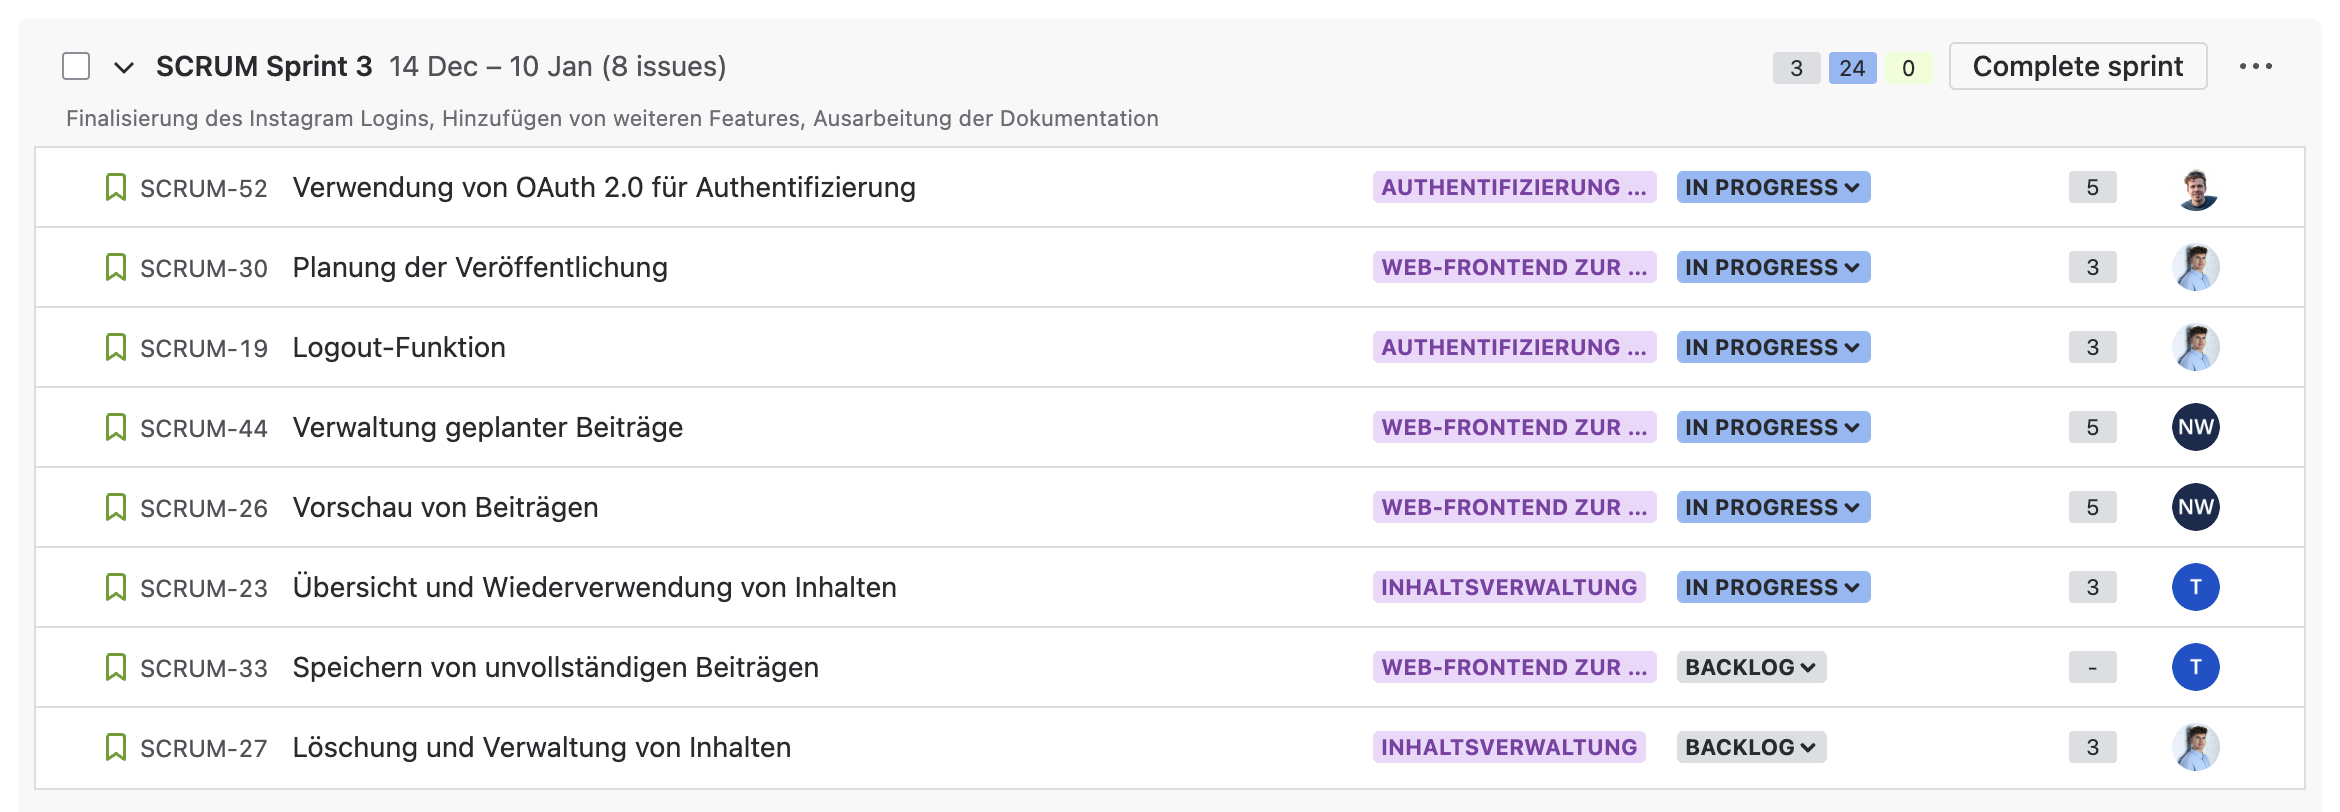
\includegraphics[width=0.8\textwidth]{graphics/sprint_3_jira.png}
    \caption{Sprint 3}
    \label{fig:fig-1}
\end{figure}

In \hyperref[fig:fig-1]{Abbildung 1} ist eine Übersicht von Sprint 3 zu sehen. Die Anzahl der Stories pro Sprint variiert je nach Komplexität und Umfang.
Die Entscheidung wie viele Stories in einen Sprint aufgenommen werden, wird im Team getroffen. Dabei wird darauf geachtet, dass die Stories in einem Sprint
realistisch umsetzbar und die Storypoints von Sprint zu Sprint annähernd gleich sind. Wird eine Storie in einem Sprint nicht fertiggestellt, wird sie in
den nächsten Sprint übernommen.

Die Definition der Anforderungen und die Planung der Sprints in Jira sind wesentliche Bestandteile des Projekts. Sie gewährleisten einen klaren Überblick über die 
Anforderungen und den Fortschritt während des gesamten Entwicklungsprozesses. Im Folgenden wird die technische Konzeption dargelegt.

\section{Technische Konzeption}
\label{sec:chapter2-1}

Im Rahmen der Entwicklung der Webanwendung wurden verschiedene Frameworks und Tools eingesetzt, um eine effiziente, flexible und 
skalierbare Lösung zu gewährleisten. Diese werden nachfolgend erläutert.

\textbf{Next.js}\footnote{Vgl. \cite{nextjs_docs}} wurde als zentrales Framework für die Entwicklung der Webanwendung verwendet. Es bietet leistungsstarke Funktionen wie Server-Side Rendering (SSR) 
und eine hohe Performance, wodurch die Ladezeiten optimiert werden. Zudem ermöglicht die Flexibilität von Next.js eine reibungslose Integration weiterer Technologien.

Für die Automatisierung der Instagram-Beiträge wird die offizielle \ac{API} von \textbf{Meta}\footnote{Vgl. \cite{facebook_graph_api}} genutzt. Diese erlaubt den Zugriff auf Beitragsdaten sowie die Planung von 
Posts, was die zentrale Funktion der Anwendung unterstützt.

Zur Implementierung einer modernen und modularen Benutzeroberfläche wurde \textbf{shadcn/ui}\footnote{Vgl. \cite{shadcn_ui_docs}} eingesetzt. Dieses UI-Framework zeichnet sich durch modulare Komponenten 
aus, die einfach erweiterbar sind. Zudem profitiert das Projekt von einer aktiven Community-Driven-Entwicklung, die regelmäßige Updates und Verbesserungen ermöglicht.

Für das Styling der Anwendung wurde \textbf{Tailwind CSS}\footnote{Vgl. \cite{tailwindcss_v2_docs}} verwendet. Der Utility-First-Ansatz erlaubt eine schnelle und konsistente Gestaltung der Benutzeroberfläche. Dank 
Responsive Design passt sich die Anwendung an verschiedene Bildschirmgrößen an. Zudem steigert Tailwind die Produktivität, da wiederverwendbare Klassen eine 
effiziente Entwicklung ermöglichen.

Zur sicheren und skalierbaren Verwaltung von Medieninhalten wurde \textbf{uploadthing} integriert. Dieses Tool bietet eine hohe Sicherheit für den Datei-Upload, eine 
nahtlose Next.js-Integration und eine gute Skalierbarkeit, um den wachsenden Anforderungen der Anwendung gerecht zu werden.

Diese beschriebenen Technologien bilden das Fundament der Webanwendung. Im nächsten Abschnitt wird die verwendete Architektur näher betrachtet.

\section{Architektur}
\label{sec:chapter2-2}

Um eine durchdachte und strukturierte Architektur zu gewährleisten, wurden zunächst verschiedene \ac{UML}-Diagramme erstellt.
Diese dienen als Grundlage für die Implementierung und ermöglichen eine klare Strukturierung, aus der die einzelnen Komponenten der Anwendung abgeleitet werden können. Durch die 
Zusammenführung dieser Komponenten entsteht die Gesamtarchitektur der Anwendung.

\begin{figure}[htb]
    \centering
    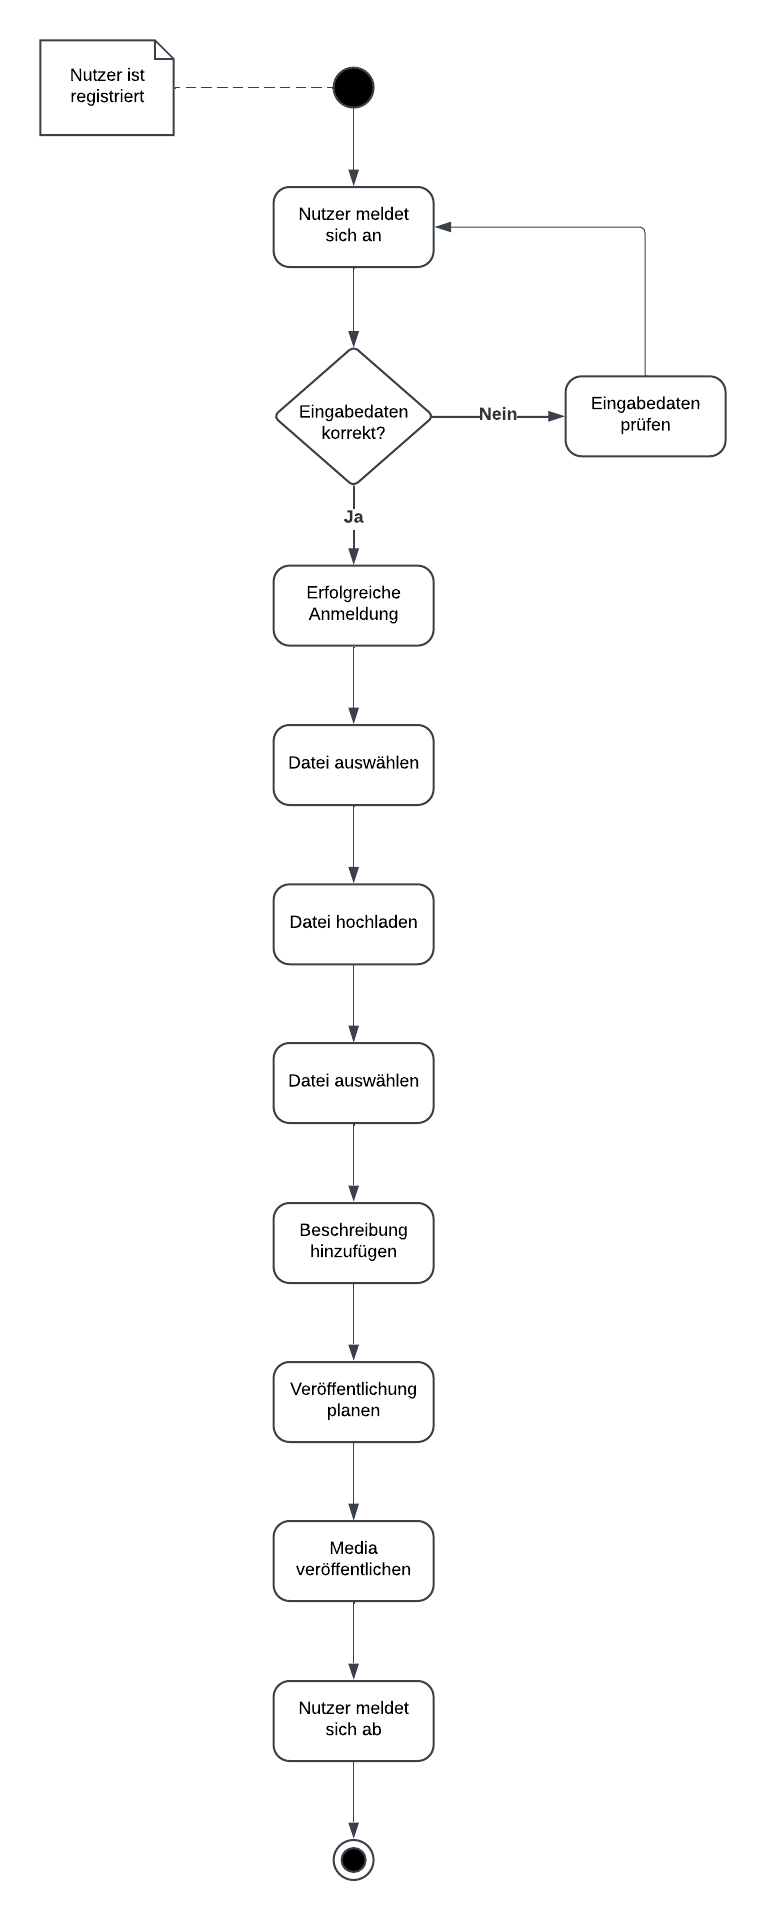
\includegraphics[width=0.8\textwidth, height=0.7\textheight]{graphics/activity_diagram.png}
    \caption[Aktivitätsdiagramm]{Aktivitätsdiagramm\footnotemark}
    \label{fig:fig-2}
\end{figure}
\footnotetext{Notation nach: \url{https://www.lucidchart.com/pages/uml-activity-diagram}}
\newpage

In \hyperref[fig:fig-2]{Abbildung 2} ist das \textbf{Aktivitätsdiagramm} dargestellt, das den typischen Ablauf der Benutzerinteraktion mit der Webanwendung zur 
automatisierten Veröffentlichung von Instagram-Beiträgen veranschaulicht. Es zeigt die einzelnen Schritte von der Anmeldung bis zur Veröffentlichung eines Beitrags 
und der anschließenden Abmeldung des Nutzers. Der Prozess beginnt mit einem bereits registrierten Nutzer, der sich in die Anwendung einloggt. Anschließend erfolgt 
eine Überprüfung der Eingabedaten. Falls diese nicht korrekt sind, wird der Nutzer zur erneuten Eingabe aufgefordert. Andernfalls erfolgt die erfolgreiche Anmeldung, 
und der Nutzer gelangt zur Hauptfunktionalität der Anwendung. Nach der Anmeldung kann der Nutzer eine Datei auswählen und diese anschließend hochladen. Dieser Schritt 
kann sich wiederholen, falls der Nutzer mehrere Dateien hochladen möchte. Anschließend wird eine Beschreibung hinzugefügt, um den Beitrag zu vervollständigen. Danach 
erfolgt die Planung der Veröffentlichung, bei der der Nutzer den gewünschten Veröffentlichungszeitpunkt festlegt. Sobald die Planung abgeschlossen ist, wird die 
Medienveröffentlichung durchgeführt. Abschließend meldet sich der Nutzer von der Anwendung ab, womit der Ablauf endet. Das Diagramm bietet eine strukturierte 
Darstellung der Benutzerinteraktion und stellt alle relevanten Schritte für eine erfolgreiche Beitragserstellung dar.

\begin{figure}[htb]
    \centering
    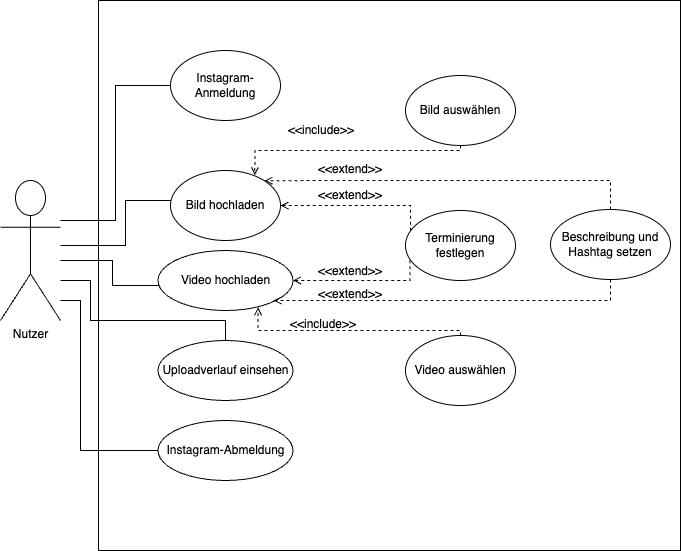
\includegraphics[width=0.8\textwidth]{graphics/use_case_diagram.png}
    \caption[Use Case Diagramm]{Use Case Diagramm\footnotemark}
    \label{fig:fig-3}
\end{figure}
\footnotetext{Notation nach: \url{https://www.lucidchart.com/pages/uml-use-case-diagram}}

\hyperref[fig:fig-3]{Abbildung 3} stellt das \textbf{Use Case Diagramm} dar, das die wesentlichen Use Cases der Webanwendung beschreibt. Es zeigt die Interaktionen 
des Nutzers mit dem System und verdeutlicht die Beziehungen zwischen den einzelnen Anwendungsfällen. Der Nutzer kann sich zunächst über die Instagram-Anmeldung in 
die Anwendung einloggen.

Nach erfolgreicher Anmeldung stehen ihm mehrere Hauptfunktionen zur Verfügung:
\begin{itemize}
    \item Bild hochladen
    \item Video hochladen
    \item Uploadverlauf einsehen
    \item Instagram-Abmeldung
\end{itemize}

Die beiden Anwendungsfälle Bild hochladen und Video hochladen beinhalten jeweils optionale Erweiterungen (\textit{<<extend>>}):
\begin{itemize}
    \item Terminierung festlegen: Der Nutzer kann den Zeitpunkt der Veröffentlichung bestimmen.
    \item Beschreibung und Hashtags setzen: Zusätzlich kann er eine Bildbeschreibung und relevante Hashtags hinzufügen.
\end{itemize}

Zudem gibt es \textit{<<include>>}-Beziehungen, die darauf hinweisen, dass bestimmte Aktionen zwingend erforderlich sind:
\begin{itemize}
    \item Bild hochladen und Video hochladen beinhalten jeweils das Auswählen einer Datei (Bild oder Video), bevor der Upload erfolgen kann.
    \item Uploadverlauf einsehen ist ein separater Use Case, der dem Nutzer ermöglicht, eine Übersicht über bereits hochgeladene Inhalte zu erhalten.
\end{itemize}

Das Diagramm visualisiert die Modularität und Erweiterbarkeit der Anwendung, indem es optionale (\textit{<<extend>>}) und zwingend notwendige (\textit{<<include>>}) 
Abhängigkeiten zwischen den Use Cases darstellt. Dadurch wird eine strukturierte und skalierbare Architektur unterstützt.

\begin{figure}[htb]
    \centering
    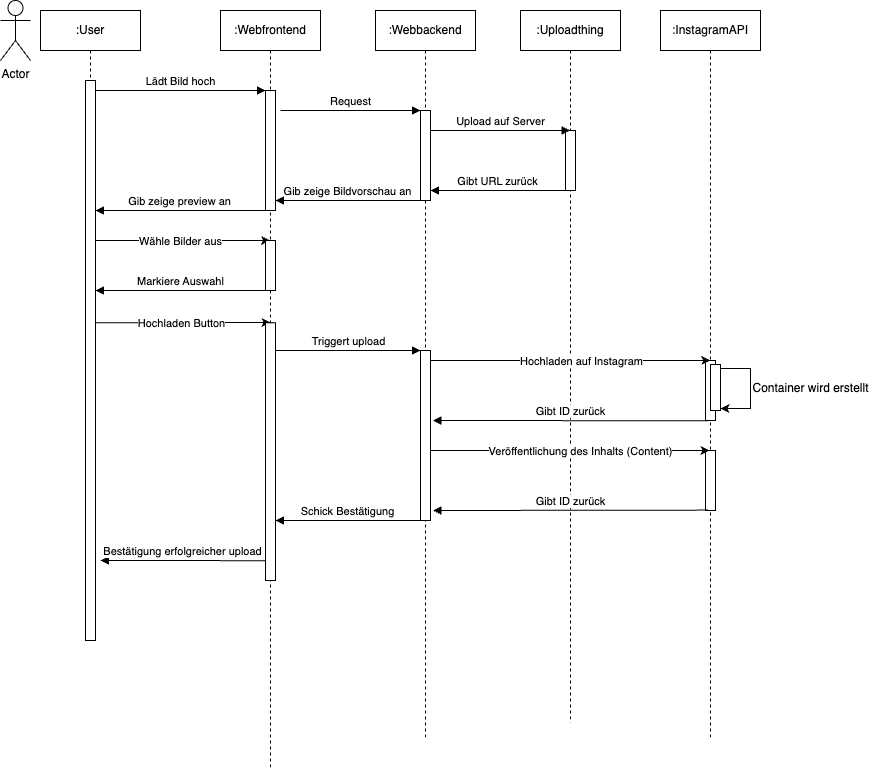
\includegraphics[width=0.8\textwidth]{graphics/sequence_diagram.png}
    \caption[Sequenzdiagramm]{Sequenzdiagramm\footnotemark}
    \label{fig:fig-4}
\end{figure}
\footnotetext{Notation nach: \url{https://www.lucidchart.com/pages/uml-sequence-diagram}}

In \hyperref[fig:fig-4]{Abbildung 4} ist das Sequenzdiagramm dargestellt, das den Ablauf für das Hochladen und Veröffentlichen eines Bildes in der Webanwendung beschreibt. Es zeigt die 
Interaktionen zwischen dem User, dem Webfrontend, dem Webbackend, dem Uploadthing-Service und der Instagram-\ac{API}. Im Folgeden wird der Ablauf der Interaktion beschrieben:

\begin{enumerate}
    \item \textbf{Nutzerinteraktion im Frontend}
    \begin{itemize}
        \item Der Nutzer lädt ein Bild hoch, indem er eine Vorschau anfordert.
        \item Das Webfrontend zeigt dem Nutzer eine Bildvorschau an, aus der er ein Bild auswählen und markieren kann.
        \item Nach Auswahl klickt der Nutzer auf den Hochladen-Button, um den Upload-Vorgang zu starten.
    \end{itemize}

\newpage

    \item \textbf{Kommunikation zwischen Frontend und Backend}
    \begin{itemize}
        \item Das Webfrontend sendet eine Request-Nachricht an das Webbackend, um den Upload-Vorgang auszulösen.
    \end{itemize}

    \item \textbf{Upload auf Uploadthing}
    \begin{itemize}
        \item Das Webbackend kommuniziert mit dem Uploadthing-Service, um die Datei auf den Server hochzuladen.
        \item Nach erfolgreichem Upload gibt Uploadthing eine URL zurück, die die hochgeladene Datei referenziert.
    \end{itemize}

    \item \textbf{Verarbeitung durch die Instagram-\ac{API}}
    \begin{itemize}
        \item Das Webbackend verwendet die Instagram-\ac{API}, um das Bild zu veröffentlichen:
        \begin{itemize}
            \item Zuerst wird ein Container erstellt, um die Metadaten des Inhalts zu speichern.
            \item Anschließend wird das Bild hochgeladen, und die ID des Containers wird zurückgegeben.
            \item Die Veröffentlichung des Inhalts erfolgt, und die Content-ID wird zurückgegeben.
        \end{itemize}
    \end{itemize}

    \item \textbf{Bestätigung des erfolgreichen Uploads}
    \begin{itemize}
        \item Nach Abschluss aller Schritte sendet das Webbackend eine Bestätigung an das Webfrontend, welches dem Nutzer den erfolgreichen Abschluss des Uploads anzeigt.
    \end{itemize}
\end{enumerate}

Das Diagramm verdeutlicht den gesamten Workflow des Upload-Prozesses, einschließlich der Interaktionen zwischen verschiedenen Systemkomponenten. Es zeigt die Synchronität der Kommunikation 
und die Abhängigkeiten zwischen Frontend, Backend, externen Services und \acp{API}. Dies unterstützt die Entwickler bei der Implementierung und Fehlerbehebung des Upload- und Veröffentlichungsprozesses.


\begin{figure}[htb]
    \centering
    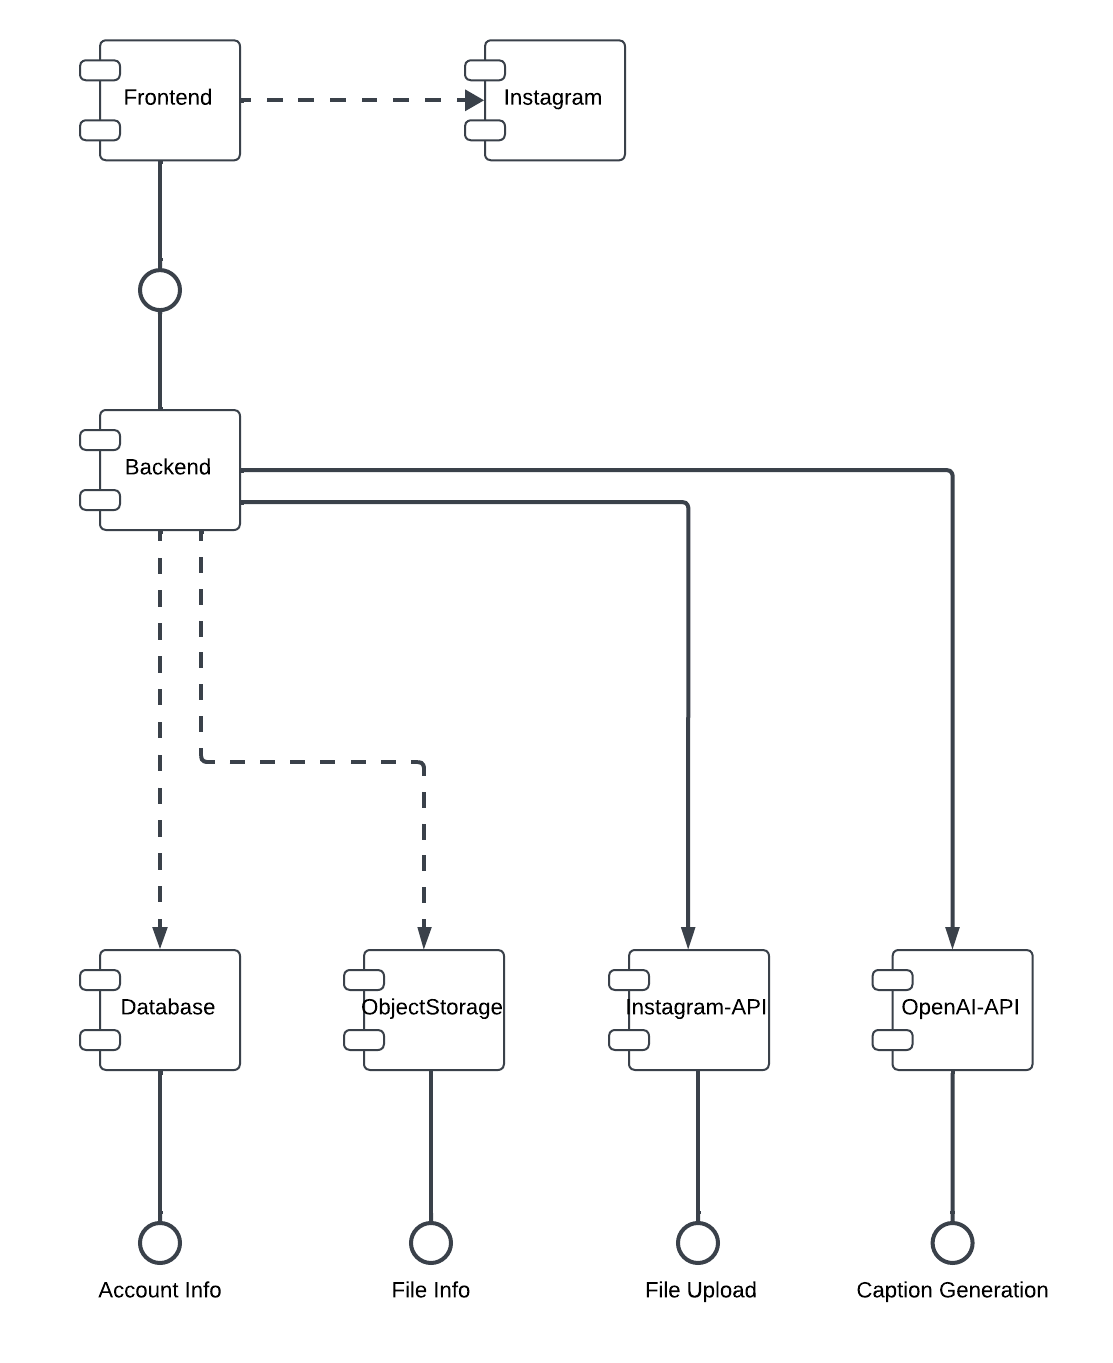
\includegraphics[width=0.8\textwidth]{graphics/components_diagram.png}
    \caption[Komponentendiagramm]{Komponentendiagramm\footnotemark}
    \label{fig:fig-5}
\end{figure}
\footnotetext{Notation nach: \url{https://www.lucidchart.com/pages/uml-component-diagram}}
\newpage

\hyperref[fig:fig-5]{Abbildung 5} zeigt das \textbf{Komponentendiagramm}, das die Architektur der Webanwendung beschreibt. Es zeigt die Hauptkomponenten sowie ihre Beziehungen und 
Abhängigkeiten zueinander. Nachfolgend werden die einzelnen Komponenten und ihre jeweiligen Funktionen beschrieben sowie die Beziehungen zwischen ihnen erläutert:

\begin{enumerate}
    \item \textbf{Frontend}
    \begin{itemize}
        \item Das Frontend stellt die Benutzeroberfläche bereit und ermöglicht die Interaktion des Nutzers mit der Anwendung.
        \item Es kommuniziert direkt mit der Instagram-Plattform, um Benutzeranmeldungen oder Beitragsvorschauen zu ermöglichen.
    \end{itemize}
    
    \item \textbf{Backend}
    \begin{itemize}
        \item Das Backend ist das zentrale Steuerungselement der Anwendung. Es verarbeitet die Daten aus dem Frontend und kommuniziert mit mehreren anderen Komponenten, darunter:
        \begin{itemize}
            \item Datenbank: Zum Speichern von Benutzerdaten, Beitragsinformationen und Metadaten.
            \item Object Storage: Für die sichere Speicherung hochgeladener Mediendateien wie Bilder oder Videos.
            \item Instagram-\ac{API}: Zum Veröffentlichen von Beiträgen oder Planen von Inhalten direkt auf Instagram.
            \item OpenAI-\ac{API}: Zur Generierung von Hashtags oder Beschreibungen basierend auf den hochgeladenen Inhalten.
        \end{itemize}
    \end{itemize}
    
    \item \textbf{Datenbank}
    \begin{itemize}
        \item Die Datenbank speichert strukturierte Daten wie Benutzerinformationen, geplante Veröffentlichungen und Protokolle der Anwendung.
    \end{itemize}
    
    \item \textbf{Object Storage}
    \begin{itemize}
        \item Der Object Storage dient der Speicherung und Verwaltung von Mediendateien wie Bildern und Videos, die mit Beiträgen verknüpft sind.
    \end{itemize}
    
    \item \textbf{Instagram-\ac{API}}
    \begin{itemize}
        \item Die Instagram-\ac{API} wird verwendet, um Inhalte auf Instagram zu veröffentlichen oder Interaktionen mit der Plattform zu ermöglichen.
    \end{itemize}
    
    \item \textbf{OpenAI-\ac{API}}
    \begin{itemize}
        \item Die OpenAI-\ac{API} wird verwendet, um KI-basierte Funktionen wie die Generierung von Textinhalten oder Vorschlägen für Hashtags bereitzustellen.
    \end{itemize}
\end{enumerate}

\textbf{Beziehungen zwischen den Komponenten}
\begin{itemize}
    \item Das Frontend kommuniziert direkt mit dem Backend, das als zentrales Gateway für alle weiteren Abhängigkeiten fungiert.
    \item Das Backend verbindet sich mit der Datenbank und dem Object Storage, um Inhalte zu speichern und zu verwalten.
    \item Die Instagram-\ac{API} und die OpenAI-\ac{API} erweitern die Funktionalität, indem sie externe Dienste integrieren.
\end{itemize}

Das Diagramm verdeutlicht die Modularität und Erweiterbarkeit der Anwendung und stellt sicher, dass die Komponenten klar voneinander getrennt sind, was die Wartbarkeit und Skalierbarkeit der 
Architektur unterstützt.




%\startAnhang

\listofanhang
\clearpage


%%% Ende des eigentlichen Inhalts %%%


%%% Quellenverzeichnisse (keine Anpassung nötig) %%%
%\clearpage
%\literaturverzeichnis
%%% Ende Quellenverzeichnisse %%%


%%% Erklärung (keine Anpassungen nötig) %%%
% steht ganz am Ende des Dokuments
\cleardoublepage
\clearpage

\thispagestyle{empty}
\DEoEN{%
{\LARGE\textsf{\textbf{Erklärung zur Verwendung generativer KI-Systeme}}\bigskip}

Bei der Erstellung der eingereichten Arbeit habe ich die nachfolgend aufgeführten auf künstlicher Intelligenz (KI) basierten Systeme benutzt:

\begin{enumerate}
\item ChatGPT-4o
\end{enumerate}

Ich erkläre, dass ich

\begin{itemize}
  \item mich aktiv über die Leistungsfähigkeit und Beschränkungen der oben genannten 
KI-Systeme informiert habe,\footnote{U.a. gilt es hierbei zu beachten, dass an KI weitergegebene Inhalte ggf. als Trainingsdaten genutzt und wiederverwendet werden. Dies ist insb. für betriebliche Aspekte als kritisch einzustufen.}
  \item die aus den oben angegebenen KI-Systemen direkt oder sinngemäß übernommenen Passagen gekennzeichnet habe,
%
% In der Fußnote Ihrer Arbeit geben Sie die KI als Quelle an, z.B.: 
% Erzeugt durch Microsoft Copilot am dd.mm.yyyy. 
% Oder: Entnommen aus einem Dialog mit Perplexity vom dd.mm.yyyy. 
% Oder: Absatz 2.3 wurde durch ChatGPT sprachlich geglättet.
%
  \item überprüft habe, dass die mithilfe der oben genannten KI-Systeme generierten und von mir übernommenen Inhalte faktisch richtig sind,
  \item mir bewusst bin, dass ich als Autorin bzw. Autor dieser Arbeit die Verantwortung für die in ihr gemachten Angaben und Aussagen trage.
\end{itemize}

Die oben genannten KI-Systeme habe ich wie im Folgenden dargestellt eingesetzt: 


\begin{tabular}{|p{4cm}|p{3cm}|p{7cm}|}
    \hline
    \textbf{Arbeitsschritt in der wissenschaftlichen Arbeit} &
%
% Beispiele hierfür sind u.a. die folgenden Arbeitsschritte: 
% Generierung von Ideen, Konzeption der Arbeit, Literatursuche, Literaturanalyse, 
% Literaturverwaltung, Auswahl von Methoden, Datensammlung, Datenanalyse, 
% Generierung von Programmcodes
%
% Wenn Sie unsicher sind, ob Sie ein verwendetes KI-System angeben müssen, 
% wenden Sie sich an Ihre:n Betreuer:in.
%
    \textbf{Eingesetzte(s) KI-System(e)} & \textbf{Beschreibung der Verwendungsweise} \\
    \hline
    Korrektur der Arbeit & ChatGPT-4o & Einzelne Kapitel ChatGPT zum Korrigieren gegeben. Erfolg: geringfügig, nach der Korrektur wurden noch einige Fehler gefunden.\\
    \hline
  \end{tabular}
} % Ende deutscher Teil
{% Beginn englische Erklaerung
{\LARGE\textsf{\textbf{Declaration on the Use of Generative AI Systems}}\bigskip}

In preparing the submitted work, I have used the following artificial intelligence (AI)-based systems:

\begin{enumerate}
\item
\item
\item \ldots
\end{enumerate}

I hereby declare that I

\begin{itemize}
  \item actively informed myself about the capabilities and limitations of the above-mentioned AI systems,\footnote{In particular, it should be noted that content passed on to AI may be used as training data and reused. This is to be considered critical, especially for operational aspects.}
  \item indicated passages directly or indirectly adopted from the above-mentioned AI systems,
%
% In the footnote of your work, cite the AI as the source, e.g.:
% Generated by Microsoft Copilot on mm.dd.yyyy. 
% Or: Taken from a dialogue with Perplexity on mm.dd.yyyy. 
% Or: Paragraph 2.3 was linguistically smoothed by ChatGPT.
%
  \item verified that the content generated and adopted by me using the above-mentioned AI systems is factually correct,
  \item am aware that as the author of this work, I bear responsibility for the statements and information provided in it.
\end{itemize}

I have utilized the above-mentioned AI systems as illustrated below: 

\begin{center}
\begin{tabular}{|p{4cm}|p{3cm}|p{7cm}|}
    \hline
    \textbf{Task in the scientific work} &
%
% Examples of such tasks include: idea generation, 
% conception of the work, literature search, literature analysis, 
% literature management, selection of methods, data collection, 
% data analysis, generation of program code
%
% If you are unsure whether you need to specify an AI system used, 
% consult your supervisor.
%
	 \textbf{AI System(s) Used} & \textbf{Description of Usage} \\
    \hline
    & & \\ % Placeholder for your entries, insert your information here
    \hline
    & & \\ % (Expand the table as needed and continue on subsequent pages)
    \hline
    & & \\
    \hline
    & & \\
    \hline
  \end{tabular}
\end{center}
}

\clearpage

\thispagestyle{empty}

{\LARGE\textsf{\textbf{\DEoEN{Erklärung}{Declaration}}}\bigskip}

% \typMeinerArbeit und \themaMeinerArbeit werden in config.tex definiert
\DEoEN{%
Ich versichere hiermit, dass ich die vorliegende Arbeit mit dem Thema: \emph{\themaMeinerArbeit} selbstständig verfasst und keine anderen als die angegebenen Quellen und Hilfsmittel benutzt habe.
Ich versichere zudem, dass die eingereichte elektronische Fassung mit der gedruckten Fassung übereinstimmt.%
}{%
I hereby insure that I have personally authored this thesis with the topic: \emph{\themaMeinerArbeit} and have used no sources and aids other than those indicated. I also insure that the submitted electronic version corresponds to the printed version.%
}

\vspace{3cm}

\begin{center}
\begin{tabular}{ccc}
(\DEoEN{Ort, Datum}{place, date}) & \hspace{0.3\linewidth} & (\DEoEN{Unterschrift}{signature})
\end{tabular}
\end{center}


\end{document}